\section{Results}
\label{sec:results}

\subsection{The decoders use the neural signal}
\label{sec:res-decoders}

Before we evaluate the trust layer, we check that each decoder reads its input (\cref{tab:decoders}). Our asynchronous MEG decoder reached a test CER of 0.506 with greedy decoding (0.495 $\pm$ 0.020 SEM over the 19 participants) and 0.475 with beam search and the character LM (\cref{fig:megcer}). With shuffled MEG the CER rose to 0.760 and with zero input to 0.925; the paired shuffled-minus-real gap was $+0.254$ \ci{+0.241}{+0.265} (instances). On the 11 test sentences with no close training variant, CER was 0.519 (greedy) and 0.492 (beam + LM), so near-variant sentences changed the headline by about 0.013 and 0.017. A longer training schedule did not help (r5 minus r4b, greedy $+0.009$ \ci{+0.003}{+0.015}). For reference, the published asynchronous encoder reports $0.59 \pm 0.02$ on SpanishBCBL \citep{zhang2026brain2qwertyv2}; this is not a head-to-head comparison, because the test splits differ and our decoder uses key times as training labels. On B2T '25, our phoneme-to-word route reached WER 0.149 and the published decoder 0.043. On sEMG, the CNN reached key accuracies of 0.299 (session-calibrated), 0.168 (cross-session) and 0.209 (cross-subject); with permuted training labels it fell to 0.022, the chance level.

\begin{table}[t]
  \centering
  \caption{\textbf{Decoder quality and input controls.} CER/WER on the test sets; lower is better. MEG intervals are over instances. ``Far'' = the 11 MEG test sentences with no close training variant.}
  \label{tab:decoders}
  \small
  \begin{adjustbox}{max width=\linewidth}\begin{tabular}{@{}llll@{}}
    \toprule
    \textbf{Device} & \textbf{Decoder} & \textbf{Real input} & \textbf{Controls} \\
    \midrule
    MEG & M1-09 async, greedy (CER) & 0.506 (participants 0.495 $\pm$ 0.020) & shuffled 0.760, zeros 0.925 \\
    MEG & M1-09 async, beam + LM (CER) & 0.475 (participants 0.462 $\pm$ 0.022) & --- \\
    MEG & far sentences, greedy / beam (CER) & 0.519 / 0.492 & --- \\
    MEG & v2 Encoder Async \citep{zhang2026brain2qwertyv2} (CER) & $0.59 \pm 0.02$ (other split) & --- \\
    B2T '25 & our phoneme-to-word route (WER) & 0.149 & --- \\
    B2T '25 & published decoder (WER) & 0.043 (0.0434 pooled, 1,718 trials) & --- \\
    sEMG & CNN, session-cal.\ / cross-session / cross-subject & key accuracy 0.299 / 0.168 / 0.209 & permuted labels 0.022 \\
    \bottomrule
  \end{tabular}\end{adjustbox}
\end{table}

\begin{figure}[t]
  \centering
  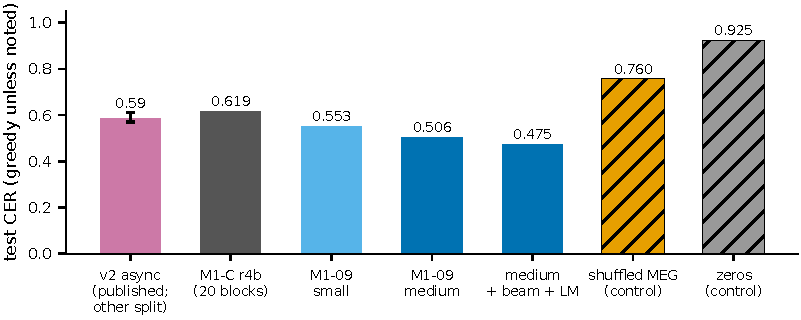
\includegraphics[width=\linewidth]{fig_meg_cer.pdf}
  \caption{\textbf{Our asynchronous MEG decoder uses the signal.} Test CER on SpanishBCBL (637 instances, 17 unique sentences, 19 participants), mean over sentences. The published v2 value (mean $\pm$ SEM over participants) uses a different test split and is shown for orientation only. Hatched bars: input controls for the medium model (greedy). \todo{G2: add seed variability.}}
  \label{fig:megcer}
\end{figure}

\subsection{The trust layer cuts wrong commits on three device types}
\label{sec:res-main}

\Cref{tab:main} and \cref{fig:teaser,fig:ewpm} give the main result.

\paragraph{Intracortical speech.} Always committing the top sentence of our decoder gave 11.45 \ewpm{} and a wrong-commit rate of 0.610. The trust layer, on the same output, gave 11.55 \ewpm{} and a wrong-commit rate of 0.059 \ci{0.043}{0.075}. The paired \ewpm{} difference was \ci{-0.11}{+0.30} and the wrong-commit difference \ci{-0.587}{-0.516} (trials). Used as a gate on the published LM-rescored sentences, the layer reduced the wrong-commit rate from 0.194 to 0.044 \ci{0.031}{0.059} at a speed cost of 4.3\% (paired \ewpm{} \ci{-0.98}{-0.72}). All BCI policies were far faster than gaze typing alone (4.08 \ewpm{}; trust minus gaze \ci{+6.96}{+7.97}, gate minus gaze \ci{+13.81}{+15.53}).

\paragraph{Forearm sEMG.} In all three decoder conditions the trust layer reduced the wrong-commit rate from 0.541, 0.882 and 0.962 to 0.004, 0.004 and 0.000, and it raised \ewpm{} over always-commit (paired differences \ci{+0.05}{+0.38}, \ci{+0.44}{+0.72} and \ci{+0.43}{+0.67}, sentences). The layer committed only 0--4\% of sentences; the speed gain came from offers, from which the user picks a candidate. Only the session-calibrated decoder clearly beat gaze typing (8.02 vs 4.27 \ewpm{}; trust minus gaze \ci{+3.38}{+4.16}). The cross-subject condition stayed below gaze typing (4.08).

\paragraph{MEG.} With our asynchronous decoder, the LM top sentence was right for 2 of 637 test instances (0.0031), and the true sentence was in the 10-best list for 1.6\%. Always committing the top sentence therefore gave a wrong-commit rate of 0.997 and 2.580 \ewpm{} \ci{2.41}{2.76}. The trust layer committed nothing (wrong-commit 0) and offered candidates instead, which gave 3.203 \ewpm{} \ci{3.07}{3.36} (sentences; \{3.08, 3.37\} over participants), $+0.62$ over always-commit \ci{+0.49}{+0.75}. Gaze typing alone gave 3.155 \ci{3.02}{3.29}. The paired difference to gaze typing was $+0.05$, with CIs of \ci{-0.04}{+0.15} over sentences and \ci{-0.07}{+0.22} over participants: this is parity, not a gain. Per participant, the trust layer was above gaze typing for 10 of 19 participants and below for 9 (range $-0.34$ to $+1.16$ \ewpm{}). The synchronous M1-15 decoder with oracle key timing gave the same picture (trust 3.229, always-commit 2.714; trust minus gaze \ci{-0.02}{+0.18} over sentences).

\begin{table}[t]
  \centering
  \caption{\textbf{Safety and speed on three device types (test sets).} \ewpm{} with 95\% bootstrap CIs; square brackets: trials (B2T '25) or sentences (sEMG; MEG, cluster bootstrap over the 17 unique sentences); curly brackets: days (B2T '25) or participants (sEMG, MEG). The MEG wrong-commit CI is over sentences. Wrong-commit: share of items committed with an error. Silent error: wrong commit not noticed by the simulated user. ``---'': not computed.}
  \label{tab:main}
  \small
  \begin{adjustbox}{max width=\linewidth}\begin{tabular}{@{}lllll@{}}
    \toprule
    \textbf{Device / condition} & \textbf{Policy} & \textbf{\ewpm{} [CI] \{CI\}} & \textbf{Wrong-commit} & \textbf{Silent} \\
    \midrule
    B2T '25, our decoder & always commit top-1 & 11.45 \ci{10.95}{12.04} \{10.72, 12.32\} & 0.610 \ci{0.574}{0.645} & 0.044 \\
     & trust & 11.55 \ci{11.03}{12.06} \{10.85, 12.38\} & 0.059 \ci{0.043}{0.075} & 0.002 \\
    B2T '25, published & always commit & 19.61 \ci{18.68}{20.51} \{17.76, 21.45\} & 0.194 \ci{0.167}{0.222} & 0.025 \\
     & trust gate & 18.77 \ci{17.88}{19.62} \{17.05, 20.46\} & 0.044 \ci{0.031}{0.059} & 0.004 \\
    B2T '25 & gaze typing only & 4.08 \ci{4.04}{4.12} & 0 & 0 \\
    \midrule
    sEMG session-cal. & always commit LM top-1 & 7.81 \ci{7.36}{8.30} \{6.60, 9.01\} & 0.541 & 0.060 \\
     & trust & 8.02 \ci{7.63}{8.45} \{6.90, 9.15\} & 0.004 & 0.000 \\
    sEMG cross-session & always commit LM top-1 & 4.10 \ci{3.89}{4.34} \{3.59, 4.70\} & 0.882 & 0.149 \\
     & trust & 4.68 \ci{4.52}{4.86} \{4.21, 5.25\} & 0.004 & 0.000 \\
    sEMG cross-subject & always commit LM top-1 & 3.53 \ci{3.37}{3.72} & 0.962 & 0.167 \\
     & trust & 4.08 \ci{3.98}{4.20} & 0.000 & 0.000 \\
    sEMG & gaze typing only & 4.27 & 0 & 0 \\
    \midrule
    MEG (async M1-09) & always commit LM top-1 & 2.580 \ci{2.41}{2.76} \{2.41, 2.79\} & 0.997 \ci{0.990}{1.000} & 0.235 \\
     & trust & 3.203 \ci{3.07}{3.36} \{3.08, 3.37\} & 0.000 & 0.000 \\
    MEG & gaze typing only & 3.155 \ci{3.02}{3.29} & 0 & 0 \\
    \bottomrule
  \end{tabular}\end{adjustbox}
\end{table}

\begin{figure}[t]
  \centering
  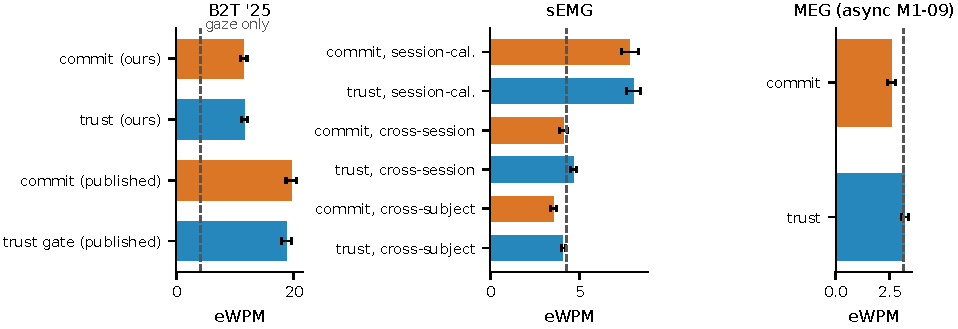
\includegraphics[width=\linewidth]{fig_ewpm_policies.pdf}
  \caption{\textbf{Speed per policy and device.} \ewpm{} of the simulated user; orange: always commit, blue: trust layer. Error bars: 95\% bootstrap CIs over trials (B2T '25) and sentences (sEMG; MEG, 17 unique sentences). Dashed lines: gaze typing alone. The trust layer never made the system slower than always-commit except for the published-decoder gate ($-4.3\%$).}
  \label{fig:ewpm}
\end{figure}

\subsection{Confidence predicts errors, and calibration helps}
\label{sec:res-calib}
On B2T '25, the calibrated top-1 probability predicted a wrong top sentence with AUROC 0.797 at the word level and 0.884 at the phoneme level; per word, the acoustic word confidence gave AUROC 0.844. The raw logits were over-confident (frame temperature 3.78); sentence ECE fell from 0.448 to 0.067. On sEMG, AUROC was 0.83, 0.76 and 0.67 in the three conditions, and sentence ECE fell from 0.154 to 0.148, from 0.328 to 0.072 and from 0.500 to 0.083 (frame temperatures 1.25, 1.78 and 2.17) (\cref{fig:ece}). \Cref{fig:risk} shows the trade-off between commit rate and wrong-commit rate as the commit threshold varies. The published B2T '25 decoder can commit about half of its sentences at the 0.05 level; our weaker decoder about a fifth; the cross-subject sEMG decoder produced no committable candidate. \todo{F5: reliability diagrams before/after need per-bin data that the committed JSON does not contain; add bins to the harness output.}

\begin{figure}[t]
  \centering
  \begin{subfigure}[t]{0.47\linewidth}
    \centering
    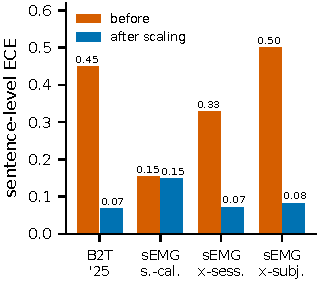
\includegraphics[width=\linewidth]{fig_ece.pdf}
    \caption{Sentence-level ECE of $\hat p_{\mathrm{top1}}$.}
    \label{fig:ece}
  \end{subfigure}\hfill
  \begin{subfigure}[t]{0.51\linewidth}
    \centering
    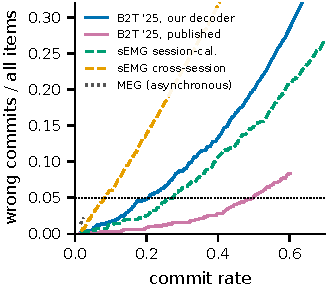
\includegraphics[width=\linewidth]{fig_risk_coverage.pdf}
    \caption{Wrong-commit rate vs commit rate.}
    \label{fig:risk}
  \end{subfigure}
  \caption{\textbf{Calibration and the commit trade-off.} (a)~Expected calibration error of the sentence confidence before and after temperature scaling (test sets). (b)~For each commit threshold on the calibrated score, the share of all test items that are committed (x) and committed wrongly (y); items blocked by the guard or other policy rules are never committed. Dotted line: $\alpha = 0.05$. The cross-subject sEMG condition is absent because no candidate passed the guard.}
  \label{fig:calib}
\end{figure}

\subsection{Null input yields no committed text}
\label{sec:res-null}
Always-commit wrote a sentence for every null input: on B2T '25 for 100\% of frame-shuffled and uniform streams, on sEMG for 100\% of frame-shuffled, zero-input and permuted-decoder streams, and on MEG for 100\% of shuffled-MEG, zero-MEG, frame-shuffled, uniform and other-sentence inputs, with fluent Spanish in 85--100\% of them (85\% on real input). The trust layer committed 0\% of null inputs on all three devices (\cref{fig:null}). On B2T '25 and sEMG this is a real test, because the same layer did commit on real input (22\% and 2.5\% of the audited items). On MEG it is not: the layer committed 0\% of real inputs as well, so the MEG audit shows that the gate stayed closed, not that it can tell null input from real input. One control it cannot pass: given the \emph{real} stream of another sentence, the trust layer on our B2T decoder committed 22\% of items, the same rate as for real input, and on sEMG it committed as often as for real input. The published-sentence gate committed 0\% in this case, because the published text did not match the other sentence's stream. A layer that sees only the stream cannot detect that the user intended a different sentence.

\begin{figure}[t]
  \centering
  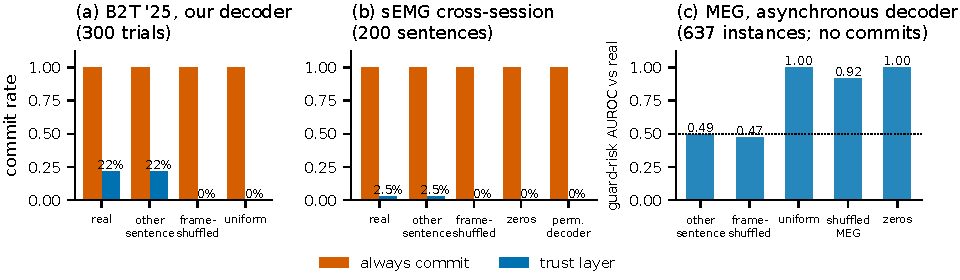
\includegraphics[width=\linewidth]{fig_null_audit.pdf}
  \caption{\textbf{Null-input audit.} Commit rate of always-commit (orange) and the trust layer (blue) on real and null inputs. (a)~B2T '25, our decoder, 300 random test trials. (b)~sEMG cross-session, 200 random test sentences. (c)~MEG, asynchronous M1-09 decoder, all 637 test instances; the trust layer also committed 0\% of real inputs, so this panel shows a closed gate, not null detection. For ``real'' and ``other sentence'', commits are a mix of right and wrong; for all other inputs any commit is wrong.}
  \label{fig:null}
\end{figure}

\subsection{Conformal risk control fixes the mean wrong-commit rate}
\label{sec:res-crc}
The plug-in policy exceeded the target on B2T '25 with our decoder (0.059 on the full test set). Over 200 random calibration/test splits with 408 calibration trials (\cref{tab:crc}, \cref{fig:crc}), CRC brought the mean test wrong-commit rate to 0.0483 (our decoder) and 0.0478 (published gate), at an \ewpm{} change of $-0.3\%$ and $+0.1\%$. LTT gave 0.0345 for both. CRC controls the mean, not every split: 41--45\% of CRC splits were above 0.05 and the 95th percentile was 0.071--0.076. LTT lowered the 95th percentile to 0.056--0.061. On MEG, where almost every possible commit is wrong, CRC still committed 2.1\% of trials (wrong-commit 0.0193; LTT 0.0214) because this is below the budget; it gained no speed (\ewpm{} 3.199 vs 3.204 for the plug-in gate, which committed nothing). Calibration splits grouped by sentence (11 of 17) or by participant (12 of 19) gave the same picture (CRC 0.0194 and 0.0201). On sEMG, with 142 calibration sentences, both methods were feasible (cross-session CRC threshold 0.204, bound 0.049) and equal to the stricter plug-in policy.

\begin{table}[t]
  \centering
  \caption{\textbf{CRC and LTT for the commit threshold} ($\alpha = 0.05$, $\delta = 0.1$, 408 calibration trials, 200 random splits). Mean over splits; p95: 95th percentile over splits. MEG: async M1-09 streams.}
  \label{tab:crc}
  \small
  \begin{adjustbox}{max width=\linewidth}\begin{tabular}{@{}llllll@{}}
    \toprule
    \textbf{Data} & \textbf{Method} & \textbf{Wrong-commit} & \textbf{p95} & \textbf{Commit rate} & \textbf{\ewpm{}} \\
    \midrule
    B2T '25, our decoder & plug-in gate & 0.0586 & 0.071 & 0.233 & 11.57 \\
     & CRC & 0.0483 & 0.071 & 0.194 & 11.53 \\
     & LTT & 0.0345 & 0.056 & 0.156 & 11.52 \\
    B2T '25, published gate & plug-in gate & 0.0441 & 0.059 & 0.471 & 18.77 \\
     & CRC & 0.0478 & 0.076 & 0.479 & 18.78 \\
     & LTT & 0.0345 & 0.061 & 0.427 & 18.70 \\
    MEG (async M1-09) & plug-in gate & 0.0000 & 0.0000 & 0.000 & 3.204 \\
     & CRC & 0.0193 & 0.0306 & 0.021 & 3.199 \\
     & LTT & 0.0214 & 0.0349 & 0.023 & 3.199 \\
    \bottomrule
  \end{tabular}\end{adjustbox}
\end{table}

\begin{figure}[t]
  \centering
  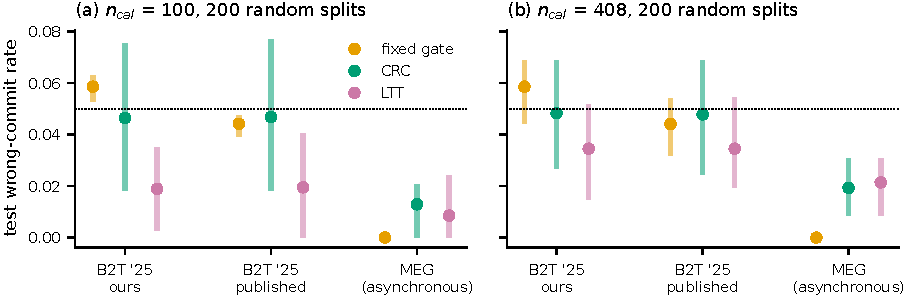
\includegraphics[width=\linewidth]{fig_crc_splits.pdf}
  \caption{\textbf{CRC controls the mean, LTT also the tail.} Test wrong-commit rate over 200 random calibration/test splits with (a)~100 and (b)~408 calibration items. Dots: mean; bars: 5th to 95th percentile. Dotted line: $\alpha = 0.05$.}
  \label{fig:crc}
\end{figure}

\subsection{Online re-calibration restores the target under drift}
\label{sec:res-drift}
CRC assumes exchangeable items. When we calibrated on the earlier half of each B2T '25 day and applied the threshold to the later half in time order, offline CRC gave 0.0625; on sEMG cross-session it gave 0.0635 (\cref{tab:drift}). The online methods brought both to 0.040--0.053 at an \ewpm{} cost of at most 0.6\%. \texttt{aci\_window} stayed below 0.05 in every drift case (0.0478 and 0.0490) and \texttt{aci} sat at the target (0.0502 and 0.0526), as its bound predicts. \Cref{fig:drift}a shows the running rate. Feedback delayed by 10 trials changed little (0.0404--0.0502 on B2T '25, our decoder). Without a calibration block (cold start over all 1,628 trials), \texttt{aci} gave 0.0442 and \texttt{aci\_window} 0.0491. No method controlled short windows: the maximum over 50-trial windows was 0.10--0.12 for all methods, as for an i.i.d.\ Bernoulli(0.05) sequence (median 0.120). When only noticed errors were fed back, \texttt{aci} gave 0.0515 on B2T '25 and 0.0635 on sEMG cross-session, because silent errors look correct to the controller.

\begin{table}[t]
  \centering
  \caption{\textbf{Wrong-commit rate under within-session drift.} Warm start on earlier data, then the later data in time order. \ewpm{} in brackets. MEG: async M1-09 streams in participant order, warm start on validation data; almost every commit is wrong. \todo{G3: CIs over days/sessions.}}
  \label{tab:drift}
  \small
  \begin{adjustbox}{max width=\linewidth}\begin{tabular}{@{}llllll@{}}
    \toprule
    \textbf{Data} & \textbf{Offline CRC} & \texttt{window} & \texttt{decay} & \texttt{aci} & \texttt{aci\_window} \\
    \midrule
    B2T '25, ours & 0.0625 (11.553) & 0.0453 (11.490) & 0.0417 (11.500) & 0.0502 (11.510) & 0.0478 (11.489) \\
    B2T '25, published & 0.0490 (18.80) & 0.0429 (18.77) & 0.0392 (18.74) & 0.0478 (18.80) & 0.0453 (18.77) \\
    sEMG cross-session & 0.0635 (4.657) & 0.0508 (4.669) & 0.0399 (4.670) & 0.0526 (4.667) & 0.0490 (4.668) \\
    MEG (async M1-09) & 0.0204 (3.198) & 0.0078 (3.201) & 0.0204 (3.198) & 0.0188 (3.200) & 0.0078 (3.201) \\
    \bottomrule
  \end{tabular}\end{adjustbox}
\end{table}

\begin{figure}[t]
  \centering
  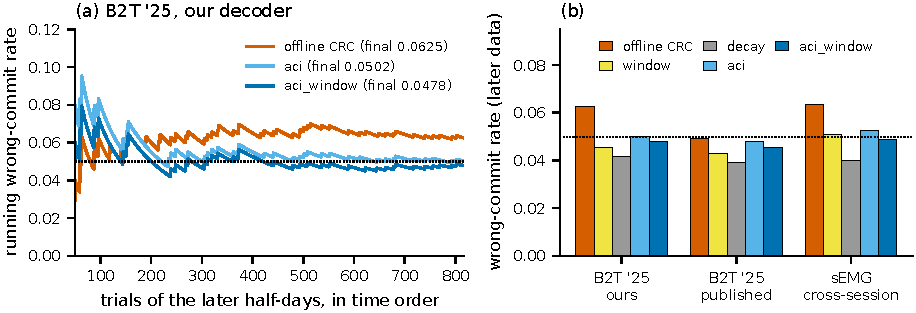
\includegraphics[width=\linewidth]{fig_drift.pdf}
  \caption{\textbf{Online re-calibration keeps the long-run rate at the target under drift.} (a)~Running wrong-commit rate over the later half-days of B2T '25 (our decoder, 816 trials, time order), recomputed from the committed per-trial items; final values equal \cref{tab:drift}. The first 50 trials are not shown. (b)~Final wrong-commit rate per method and dataset. Dotted line: $\alpha = 0.05$.}
  \label{fig:drift}
\end{figure}

\paragraph{Two CRC numbers on sEMG.} \Cref{sec:res-crc} reports a wrong-commit rate of 0.004 for CRC on sEMG cross-session, and \cref{tab:drift} reports 0.0635. Both are correct. The first combines CRC with the stricter \ewpm{}-tuned threshold ($\max(\lambda_{\mathrm{tuned}}, \hat\lambda_{\mathrm{CRC}})$); the second uses the pure CRC threshold, which exposes the drift that the stricter threshold hid.

\subsection{The ledger traces every wrong commit}
\label{sec:res-ledger}
We replayed the B2T '25 test half (816 trials) with the ledger attached, for the plug-in gate and a CRC gate. The ledger held 1,723 entries and passed verification. It found the same wrong commits as the harness: 48 of 48 (plug-in) and 39 of 39 (CRC), of which 2 and 1 were silent. Every tampering case we tried was detected: editing an entry, editing with re-hashing, deleting, reordering, and cutting the tail (with the head anchor). The cost was about 0.1\,ms and about 1.1\,kB per decision. \Cref{fig:audit} shows one entry of the audit report: most wrong commits were one-word errors.

\subsection{Ablations}
\label{sec:res-ablation}
On B2T '25, removing calibration raised the wrong-commit rate from 0.059 to 0.071 (\ewpm{} 11.57 vs 11.55), and removing the guard lowered it to 0.036 (\ewpm{} 11.51): the guard did not help on this device. On sEMG session-calibrated, removing calibration raised the wrong-commit rate from 0.004 to 0.045 and \ewpm{} from 8.02 to 8.15. \todo{G5: one unified ablation table over the three devices (calibration, guard, conformal sets, \act{offer\_words}, CRC on/off), same seeds.}

\begin{figure}[t]
  \centering
  \fbox{\begin{minipage}{0.94\linewidth}\footnotesize\raggedright
  \textbf{Wrong commit} \texttt{dec-000041-ed60b4bd} (entry 44, hash \texttt{8cf2c6c67053b185...})\\
  Committed: ``who you never expect to when''\\
  Correction (oracle ground truth, hash-linked): ``who you never expect to win''; 2 character edits, 1 word edit\\
  Scores: $\hat p_{\mathrm{top1}}$ 0.5814, set size 3, guard risk 0.2857; reason: $\hat p_{\mathrm{top1}} \ge 0.50$\\
  Input: stream \texttt{1b4b60e8e4950710...}, frames [0, 335], item \texttt{b2t25-test-trial-196}\\
  Decoder: published online RNN + our phoneme-to-word decoder; LM: Tatoeba character 6-gram + word unigram + CMUdict; adapter \texttt{fidetype.adapters.b2t25}\\
  Calibration \texttt{cal-692fb52a73417552}: $T_f$ 3.7809, $T_s$ 4.5551, fit set: first half of each day (812 trials)\\
  Policy \texttt{pol-2eaa4ff51919527a}: commit threshold 0.5, maximum guard risk 0.5, offer size 2
  \end{minipage}}
  \caption{\textbf{One entry of the provenance audit report} (B2T '25 replay, plug-in gate; public CC0 cue sentence). Each wrong commit is traced to the exact stream segment and to the decoder, LM, calibration and policy versions that produced it. Hashes are shortened.}
  \label{fig:audit}
\end{figure}
